\documentclass{article}
\usepackage{pgfplots}
\pgfplotsset{compat=1.18, every axis plot/.append style={thick}}
\begin{document}
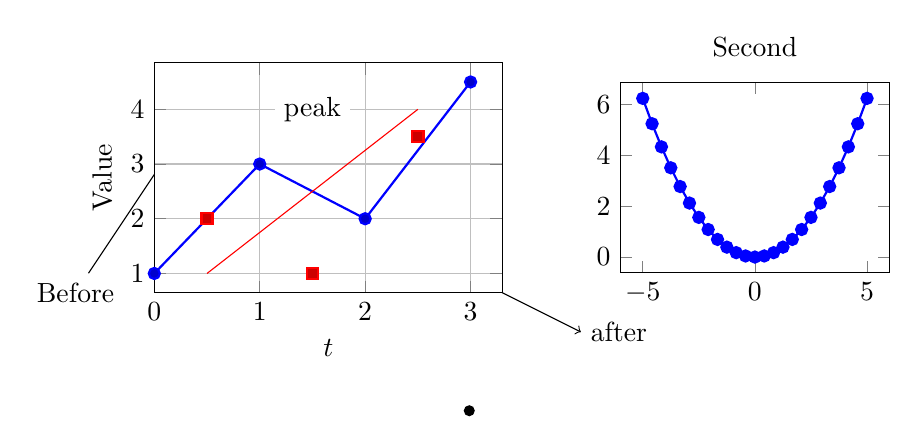
\begin{tikzpicture}
  \node (before) at (-1,0) {Before};
  \draw (before) -- (0,1.5);
  \begin{axis}[name=ax, width=6cm, height=4.5cm, xlabel={$t$}, ylabel={Value}, grid=major, xmin=0]
    \addplot coordinates {(0,1) (1,3) (2,2) (3,4.5)};
    \addplot+[only marks] table {
      x y
      0.5 2
      1.5 1
      2.5 3.5
    };
    \draw[red] (axis cs:0.5,1) -- (2.5,4);
    \node[fill=white] at (1.5,4) {peak};
  \end{axis}
  \draw[->] (ax.south east) -- ++(1,-0.5) node[right] {after};
  \begin{axis}[at={(ax.east)}, anchor=west, xshift=1.5cm, width=5cm, height=4cm, title={Second}]
    \addplot[blue, mark=*] {x^2/4};
  \end{axis}
  \fill (4,-1.5) circle (2pt);
\end{tikzpicture}
\end{document}
